\documentclass{beamer}

\usepackage{fancybox}
\usepackage{url}
% \usepackage{latexsym}
\usepackage{multirow}
% \usepackage{amsfonts,amssymb,amsthm,amsmath}
\usepackage[makeroom]{cancel}
% \usepackage{bussproofs}
\usepackage{ulem}
% \usepackage[latin1]{inputenc}
\usepackage{ifthen}
\usepackage{pgf}
% \usepackage{times}
% \usepackage[T1]{fontenc}
\usepackage{amsthm,amsmath}
\usepackage{etex}
% \usepackage{tabularx}
\usepackage{listings}
% \usepackage[all]{xy}
%\input taylor.tex

\usepackage{tikz}
\usetikzlibrary{shapes,backgrounds,arrows,automata,positioning,calc}
\tikzset{
  modal/.style={>=stealth',shorten >=1pt,shorten <=1pt,auto,node distance=1.5cm,
    semithick},
  world/.style={circle,draw,minimum size=0.5cm,fill=gray!15},
  point/.style={circle,draw,inner sep=0.5mm,fill=black},
  reflexive above/.style={->,loop,looseness=7,in=120,out=60},
  reflexive below/.style={->,loop,looseness=7,in=240,out=300},
  reflexive left/.style={->,loop,looseness=7,in=150,out=210},
  reflexive right/.style={->,loop,looseness=7,in=30,out=330}
}

\hypersetup{
    colorlinks=true,
    linkcolor=blue,
    filecolor=magenta,      
    urlcolor=cyan}
  

\definecolor{ceruleanblue}{rgb}{0.16, 0.32, 0.75}

\title[PHP]{Princípio da casa dos pombos}
\author{Alexandre Rademaker}
\institute[FGV]{FGV/EMAp, Brazil}
\date{MD 2019.2}


\begin{document}

\usebackgroundtemplate{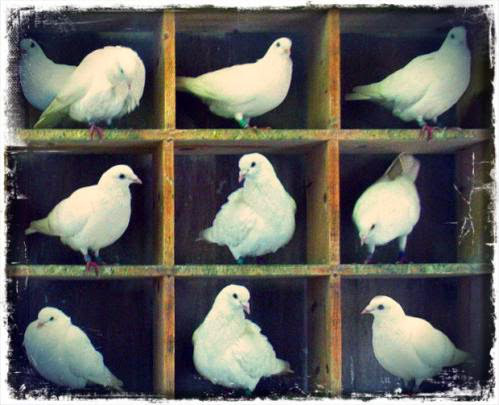
\includegraphics[width=\paperwidth]{ducking-pigeonholing.jpg}}
\setbeamercolor{normal text}{fg=white}
\setbeamercolor{title}{fg=white}
\usebeamercolor[fg]{normal text}
\frame{\textbf{\titlepage}}
\usebackgroundtemplate{}
\setbeamercolor{normal text}{fg=black}
\setbeamercolor{frametitle}{fg=ceruleanblue}
\usebeamercolor[fg]{normal text}


\begin{frame}{O princípio}

  Imagine que eu tenho 3 casas de pombos. Se eu possuo 4 pombos, então
  certamente em alguma casa haverá mais de um pombo. Se a quantidade
  de pombos é maior que a quantidade de casas, haverá certamente
  alguma casa com mais de um pombo. Foi pensando em exemplos como este
  que o princípio é chamado de Princípio da Casa dos Pombos.

  \vspace{.5cm}

  \url{https://www.youtube.com/watch?v=pPuvnD4PYNE&t=200s}\\
  \url{https://www.youtube.com/watch?v=2-mxYrCNX60}
\end{frame}


\begin{frame}{aplicação I}

  Em uma gaveta, há 4 meias pretas, 2 meias brancas, 8 meias
  cinzas. Qual é a quantidade mínima de meias que preciso retirar
  desta gaveta para garantir que terei pelo menos duas meias de cores
  diferentes?\\~\

  Vamos pensar na pior das hipóteses? Se estou querendo retirar duas
  meias de cores diferentes, o azar é pegar várias meias da mesma
  cor. Eu começo a pegar meias cinzas (porque é a que tem maior
  quantidade). Sou tão azarado que pego 8 meias cinzas
  consecutivamente.\\~\

  Depois que pego 8 meias cinzas, não tem como escapar. A próxima meia
  tem que ser de outra cor. Portanto, 9 meias é a quantidade mínima de
  meias para garantir que teremos pelo menos duas meias de cores
  distintas. Pode até ser que das 9 meias eu tenha mais de duas meias
  com cores diferentes, mas isso é sorte e não certeza.
\end{frame}

\begin{frame}{aplicação II}

  Quantas pessoas precisa haver em um auditório para ter certeza de
  que pelo menos duas delas fazem aniversário no \emph{mesmo} dia?\\~\

  Estamos procurando ter \emph{certeza}. E havendo 2 pessoas no
  auditório nunca poderíamos ter certeza de que ambas nasceram no
  mesmo dia. Com 365 pessoas no auditório, ainda não estaríamos em
  condições de assegurar que duas delas fazem aniversário no mesmo
  dia. \\~\

  No entanto, existe um argumento categórico: se houver 367 pessoas no
  auditório, não há como fugir: pelo menos duas têm de fazer
  aniversário no mesmo dia.
\end{frame}

\begin{frame}{aplicação III}{estagiários: problema}

  Um grupo de 6 estagiários foi designado para rever 50 processos e
  cada processo deveria ser revisto por apenas um dos estagiários. No
  final do trabalho, todos os estagiários trabalharam e todos os
  processos foram revistos. É correto afirmar que:\\~\

  \begin{enumerate}
  \item um dos estagiários reviu 10 processos;
  \item todos os estagiários reviram, cada um, pelo menos 5 processos;
  \item um dos estagiários só reviu 2 processos;
  \item quatro estagiários reviram 7 processos e dois estagiários
    reviram 6 processos;
  \item pelo menos um dos estagiários reviu 9 processos ou mais.
  \end{enumerate}
\end{frame}

\begin{frame}{aplicação III}{estagiários: solução}

  (A) um dos estagiários reviu 10 processos. Seria possível 5
  estagiários analisando 1 processo cada um e o sexto analisando 45
  processos. Muitas outras situações tornam a alternativa A falsa.\\~\

  (B) todos os estagiários reviram, cada um, pelo menos 5 processos;
  Não podemos garantir. Basta raciocinar da mesma maneira que a letra
  A.  Com o mesmo raciocínio percebemos que as alternativas C e D são
  falsas.\\~\

  (E) pelo menos um dos estagiários reviu 9 processos ou mais. Neste
  caso a pior das hipóteses é colocar cada estagiário para trabalhar
  com no máximo 8 processos. Como são 6, $6 \times 8 = 48$. Alguém
  terá que trabalhar com mais de 8 processos. Portanto, pelo menos um
  dos estagiários reviu 9 processos ou mais.
\end{frame}



\begin{frame}{formalização em LP}{Question \href{https://math.stackexchange.com/questions/1527273/pigeonhole-principle-formula-using-propositonal-logic}{math.stackexchange.com}}
  
Todo pombo está em uma casa (A):
$$
\bigwedge_{i=1}^{n+1}\bigvee_{j=1}^n p_{i,j},
$$

Em alguma casa temos dois pombos distintos (B)
$$
\bigvee_{j=1}^n\bigvee_{1\leq i<k\leq n+1}(p_{i,j}\land p_{k,j}).
$$

O principio é uma implicação $A \to B$. Porém, algumas pessoas
entendem que existe uma condição extra de que cada pombo está em
\textbf{apenas} uma casa! É necessário?
$$
\bigwedge_{i=1}^{n+1}\bigwedge_{1\leq j<k\leq n}\neg(p_{i,j}\land p_{i,k}).
$$
\end{frame}

\begin{frame}[fragile]{Instância $PHP_3$}{formalização SNARK}

  $PHP_2$ é trivial! Então vamos olhar para $PHP_3$ \\~\
  
\begin{lstlisting}[language=Lisp,basicstyle=\ttfamily\footnotesize]
(ql:quickload :snark)
(in-package :snark-user)

(initialize)
(use-resolution t)

(prove
 '(implies
    (and (or P11 P12) (or P21 P22) (or P31 P32))
    (or (or (and P11 P21) (and P11 P31) (and P21 P31))
        (or (and P12 P22) (and P22 P32) (and P12 P32)))))
\end{lstlisting}
\end{frame}


\begin{frame}[fragile]{Instância $PHP_3$}{Sequent Calculus and ND}

  \url{http://logitext.mit.edu/logitext.fcgi/tutorial}\\
  \url{http://logitext.mit.edu/main}\\
  \url{https://en.wikipedia.org/wiki/Natural_deduction}\\~\

  ND intro $\to$ left rules\\
  ND eliminação $\to$ right rules\\~\

  \begin{lstlisting}[basicstyle=\ttfamily\footnotesize]
  ((P11 \/ P12) /\ (P21 \/ P22) /\ (P31 \/ P32)) ->
  ((P11 /\ P21) \/ (P21 /\ P31) \/ (P11 /\ P31) \/
   (P12 /\ P22) \/ (P22 /\ P32) \/ (P12 /\ P32))
 \end{lstlisting}
\end{frame}


\begin{frame}[fragile]{Instância $PHP_3$}{Lean}

  Como? Trabalhoso mas não difícil!

\end{frame}

\end{document}

%%% Local Variables:
%%% mode: latex
%%% TeX-master: t
%%% End:
